        \documentclass[12pt]{article}

        \usepackage{sbc-template}

        \usepackage{graphicx,url}

        %\usepackage[brazil]{babel}
        \usepackage[latin1]{inputenc}


        \sloppy

        \title{Uma an�lise de pad�es em senhas}

        \author{Marino Souza S., Nilton V. C. J�nior, Luiz R. Rios}

        \address{Instituto de Matem�tica -- Universidade Federal da Bahia
          (UFBA)\\
          \email{\{marino, niltonvasques\}@openmailbox.org, luizromario@gmail.com}
        }

        \begin{document}

        \maketitle

        \begin{abstract}
          Lorem ipsum dolor sit amet, consectetur adipisicing elit, sed do eiusmod
          tempor incididunt ut labore et dolore magna aliqua. Ut enim ad minim veniam,
          quis nostrud exercitation ullamco laboris nisi ut aliquip ex ea commodo
          consequat. Duis aute irure dolor in reprehenderit in voluptate velit esse
          cillum dolore eu fugiat nulla pariatur. Excepteur sint occaecat cupidatat non
          proident, sunt in culpa qui officia deserunt mollit anim id est laborum.
        \end{abstract}

        \begin{resumo}
          Lorem ipsum dolor sit amet, consectetur adipisicing elit, sed do eiusmod
          tempor incididunt ut labore et dolore magna aliqua. Ut enim ad minim veniam,
          quis nostrud exercitation ullamco laboris nisi ut aliquip ex ea commodo
          consequat. Duis aute irure dolor in reprehenderit in voluptate velit esse
          cillum dolore eu fugiat nulla pariatur. Excepteur sint occaecat cupidatat non
          proident, sunt in culpa qui officia deserunt mollit anim id est laborum.
        \end{resumo}


        \section{Introdu��o}

        O m�todo de adivinha��o de senhas por for�a bruta necessita de um bom dicion�rio a fim de conseguir o maior n�mero de advinha��es poss�veis. Motivando-se no trabalho de \cite{chinas}, os autores deste trabalho apresentam estat�sticas de padr�es mais comuns em suas bases de dados, com o objetivo de contribuir para que dicin�rio melhores sejam criados e pol�ticas de senhas sejam fortalecidas.

        introdu��o das bases de dados, as inconsist�ncias que tinham, de onde vieram, total de cada base, total geral, e o total geral ap�s a limpesa de senhas bugadas
        Conferences that publish just abstracts ask for \textbf{one}-page texts.

        \section{Estat�sticas Comuns} \label{sec:firstpage}

        fazer uma explica��o da sess�o.

        \begin{table}[ht]
            \centering
            
            \begin{tabular}{clr}
                \hline
                & Skull leak & BR army\\
                \hline
                1 & 123456(0.202\%) & 12345678(4.864\%)\\
                2 & password1(0.119\%) & 123456789(1.009\%) \\
                3 & fuck(0.092\%) & 87654321(0.230\%)\\
                4 & abc123(0.090\%) & 10203040(0.204\%)\\
                5 & fuckyou(0.064\%) & 06121966(0.153\%)\\
                \hline
            \end{tabular}

            \caption{texto da tabela}
            \label{table:tablegeneral}

        \end{table}

        Explicar oq a tabela \ref{table:tablegeneral} significa.
        %B�nh H�a Massacre, Guerra do vietnam 6 de dezembro de 1966

        The abstract and ``resumo'' (if is the case) must be in 12 point Times font,
        indented 0.8cm on both sides. The word \textbf{Abstract} and \textbf{Resumo},
        should be written in boldface and must precede the text.

        \subsection{Subsections}

        The subsection titles must be in boldface, 12pt, flush left.

\begin{table}[h]
    \centering

    \begin{tabular}{r r r r r r}
        \hline
        & Exatamente Oito Digitos & Data valida & YYYYMMDD & MMDDYYYY & DDMMYYYY\\
        \hline
        Skull-leak & 638(0.990\%) & 219(0.340\%) & 19(8.676\%) & 37(16.894\%) & 163(74.492\%)\\
        \hline
        BrArmy & 4,565(45.513\%) & 1365(17.426\%) & 25(1.832\%) & 380(27.839\%) & 960(70.330\%)\\
        \hline
    \end{tabular}

    \caption{texto da tabela}
    \label{table:table-date}

\end{table}


\section{Figures and Captions}\label{sec:figs}


Figure and table captions should be centered if less than one line
(Figure~1), otherwise justified and indented by 0.8cm on
both margins, as shown in Figure~2. The caption font must
be Helvetica, 10 point, boldface, with 6 points of space before and after each
caption.

% \begin{figure}[ht]
% \centering
% 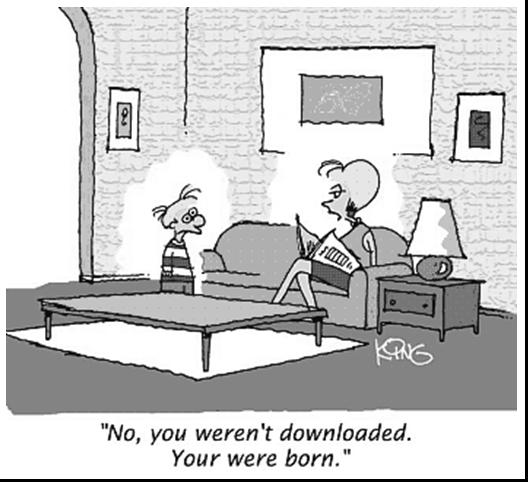
\includegraphics[width=.5\textwidth]{fig1.jpg}
% \caption{A typical figure}
% \label{fig:exampleFig1}
% \end{figure}

In tables, try to avoid the use of colored or shaded backgrounds, and avoid
thick, doubled, or unnecessary framing lines. When reporting empirical data,
do not use more decimal digits than warranted by their precision and
reproducibility. Table caption must be placed before the table (see Table 1)
and the font used must also be Helvetica, 10 point, boldface, with 6 points of
space before and after each caption.

\section{References}

Bibliographic references must be unambiguous and uniform.  We recommend giving
the author names references in brackets, e.g. \cite{knuth:84},
\cite{boulic:91}, and \cite{smith:99}.

\bibliographystyle{sbc}
\bibliography{referencias}

\end{document}
